% ── S.8 Qualitative Analysis ─────────────────────────────────────────────
\clearpage
\section*{S.8\quad Qualitative Analysis: Representative PASS Predictions}
\label{sec:s8}

Figures~\ref{fig:s8_pass_1}--\ref{fig:s8_pass_3} present twelve representative PASS predictions produced by the v0.7.3 pipeline (Quality Guard \(\theta_{\mathrm{low}}=30\), \(\theta_{\mathrm{high}}=200\)). Images are selected to cover a range of structural members and damage types. Each sub-caption shows the full original inspection record (\textbf{GT}), the full VLM-generated description (\textbf{Pred}), and sentence-embedding / TF-IDF cosine similarities (\textit{Sim(emb)} / \textit{Sim(tfidf)}). Shared damage/member terms are highlighted in bold.

\begin{figure}[H]
  \centering
  \begin{minipage}[t]{0.46\textwidth}
    {\centering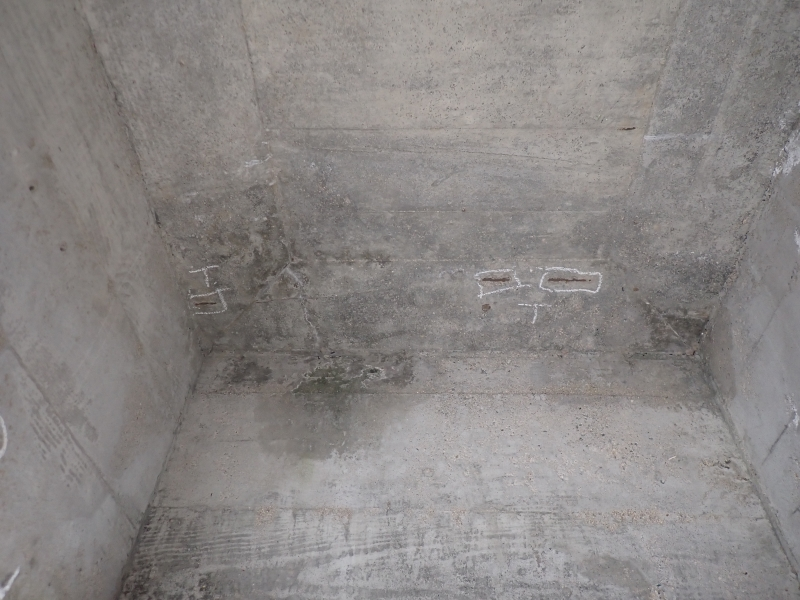
\includegraphics[width=0.75\linewidth]{figures_vlm/s8/s8_01_girder_cracking.jpg}\par}
    \vspace{2pt}
    {\scriptsize\raggedright
    \textbf{Quality Metrics:}~\textit{Sim(emb):~0.394,\;Sim(tfidf):~0.131}\\[2pt]
    \textbf{GT:} \textbf{main girder} cracking(max W=0.6mm), cross beam cracking(max W=0.25mm), deck slab cracking(W=0.2mm); \textbf{lime \textbf{efflorescence}} observed. cracking , drying shrinkage ; ASR .\\[2pt]
    \textbf{Pred:} \textbf{main girder} rebar exposure observed. Also, filler zone , \textbf{lime \textbf{efflorescence}} is present. localized , joint .
    \par}
  \end{minipage}
  \hfill
  \begin{minipage}[t]{0.46\textwidth}
    {\centering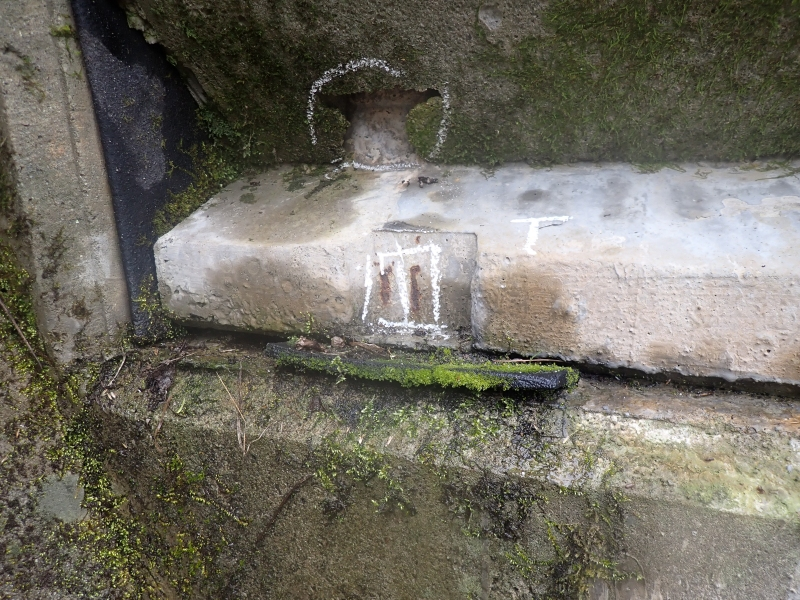
\includegraphics[width=0.75\linewidth]{figures_vlm/s8/s8_02_girder_rebar_exposure.jpg}\par}
    \vspace{2pt}
    {\scriptsize\raggedright
    \textbf{Quality Metrics:}~\textit{Sim(emb):~0.400,\;Sim(tfidf):~0.170}\\[2pt]
    \textbf{GT:} RCT girder, cross beam and deck slab \textbf{delamination}, \textbf{rebar exposure} . joint \textbf{main girder} delamination . RCT girder and deck slab spalling corrosion .\\[2pt]
    \textbf{Pred:} \textbf{main girder} \textbf{rebar exposure} observed. Also, parapet/overhang \textbf{delamination} water leakage observed. parapet , drying shrinkage insufficient cover . localized .
    \par}
  \end{minipage}
  \\[8pt]
  \begin{minipage}[t]{0.46\textwidth}
    {\centering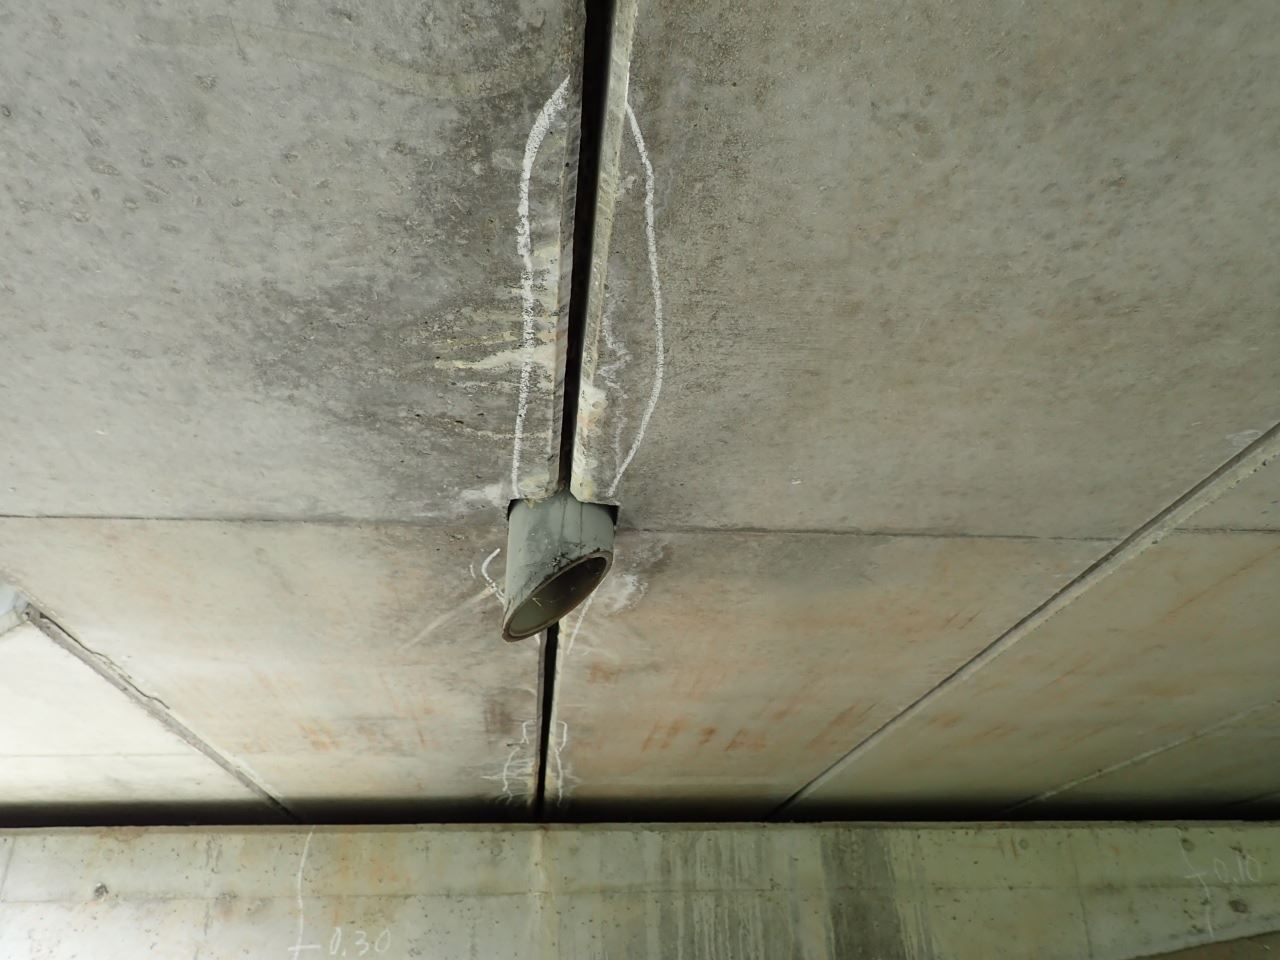
\includegraphics[width=0.75\linewidth]{figures_vlm/s8/s8_03_girder_spalling.jpg}\par}
    \vspace{2pt}
    {\scriptsize\raggedright
    \textbf{Quality Metrics:}~\textit{Sim(emb):~0.668,\;Sim(tfidf):~0.238}\\[2pt]
    \textbf{GT:} \textbf{main girder} \textbf{delamination}, corrosion, water leakage trace observed. repair as needed.\\[2pt]
    \textbf{Pred:} \textbf{main girder} rebar exposure observed. Also, parapet/overhang \textbf{delamination} rebar exposure observed. periodic monitoring;, repair if necessary .
    \par}
  \end{minipage}
  \hfill
  \begin{minipage}[t]{0.46\textwidth}
    {\centering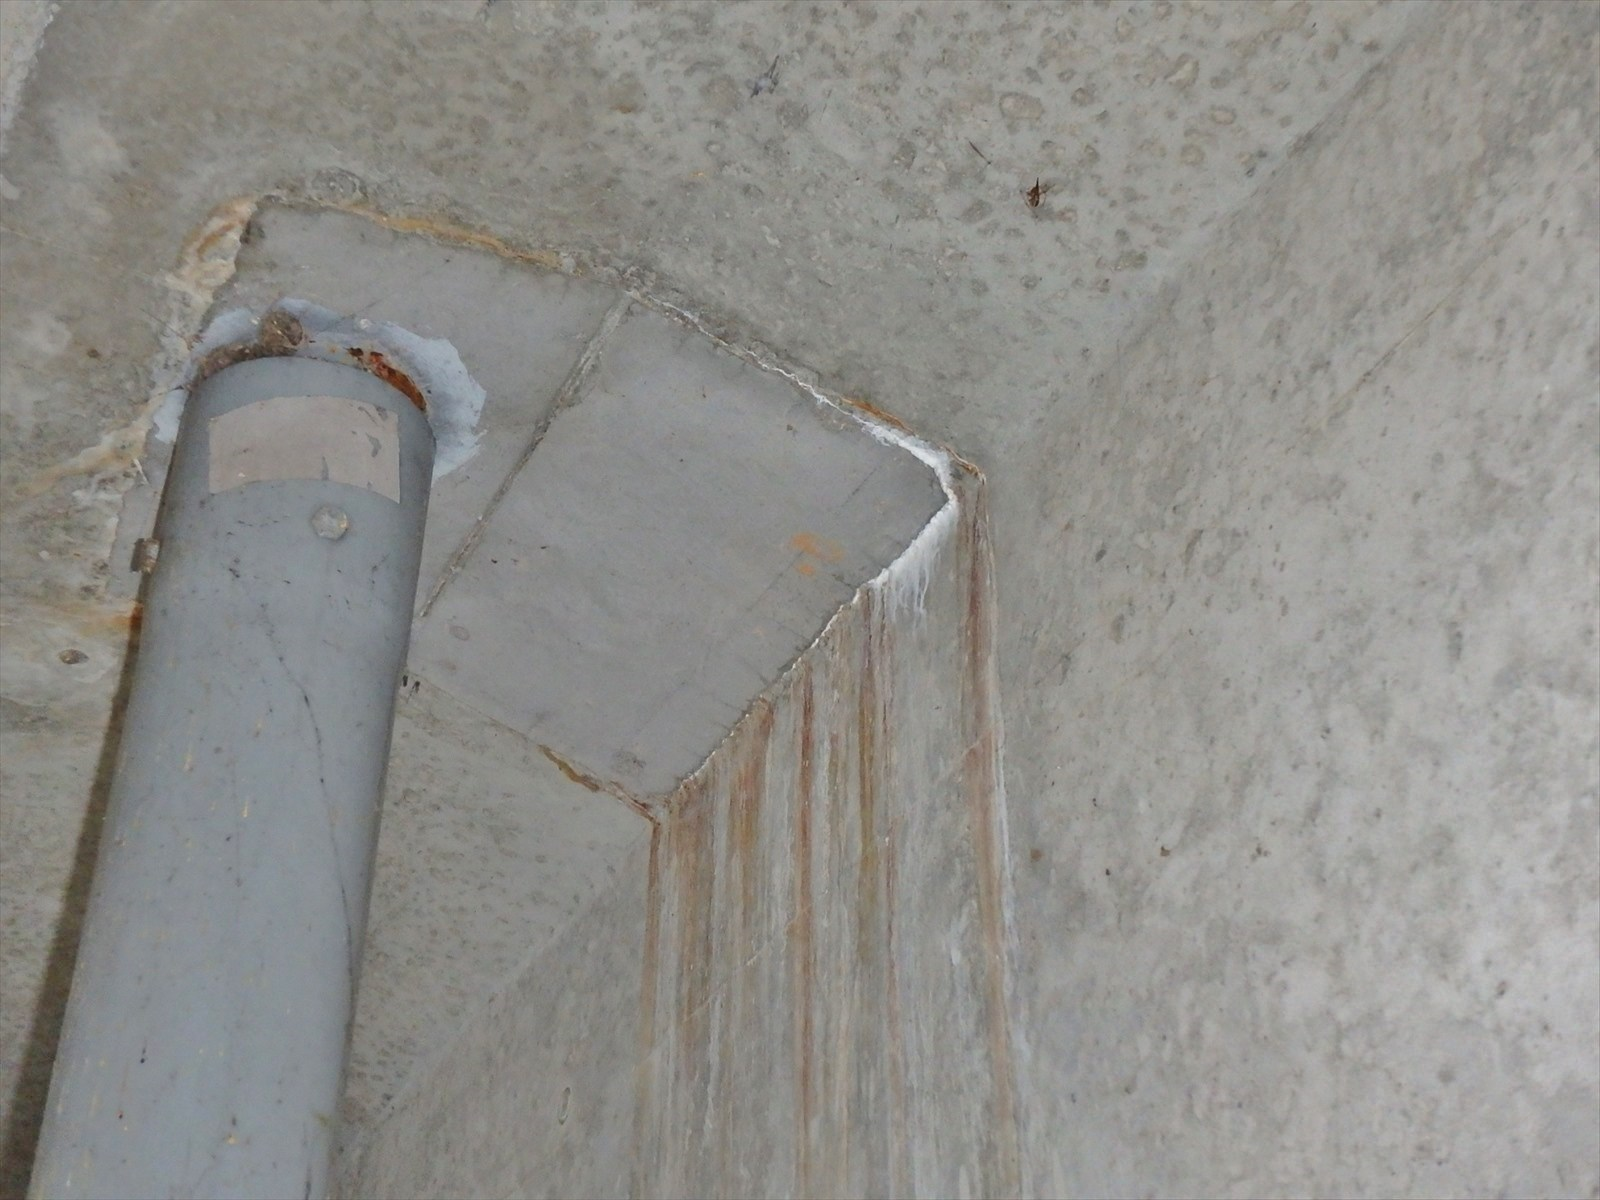
\includegraphics[width=0.75\linewidth]{figures_vlm/s8/s8_04_girder_corrosion.jpg}\par}
    \vspace{2pt}
    {\scriptsize\raggedright
    \textbf{Quality Metrics:}~\textit{Sim(emb):~0.397,\;Sim(tfidf):~0.161}\\[2pt]
    \textbf{GT:} ; \textbf{main girder} expansion joint water leakage due tosection thinning corrosion observed. Also, splice bolt corrosion observed. ; cross beam age-related deterioration due to corrosion due to observed.\\[2pt]
    \textbf{Pred:} \textbf{main girder} rebar exposure observed. Also, parapet/overhang delamination rebar exposure observed. periodic monitoring;, repair if necessary .
    \par}
  \end{minipage}
  \caption{Representative PASS predictions from the v0.7.3 pipeline (1/3). Each panel shows \textbf{GT} (full original inspection record), \textbf{Pred} (full VLM-generated description), and cosine similarities: \textit{Sim(emb)} (sentence-embedding) / \textit{Sim(tfidf)} (TF-IDF). Shared terms are in bold.}
  \label{fig:s8_pass_1}
\end{figure}
\clearpage
\begin{figure}[H]
  \centering
  \begin{minipage}[t]{0.46\textwidth}
    {\centering\includegraphics[width=0.75\linewidth]{figures_vlm/s8/s8_05_girder_leakage.jpg}\par}
    \vspace{2pt}
    {\scriptsize\raggedright
    \textbf{Quality Metrics:}~\textit{Sim(emb):~0.504,\;Sim(tfidf):~0.197}\\[2pt]
    \textbf{GT:} \textbf{main girder} cracking drying shrinkage due toage-related deterioration . main girder water leakage main girderjoint age-related deterioration .\\[2pt]
    \textbf{Pred:} \textbf{main girder} rebar exposure observed. Also, parapet , (localized) .
    \par}
  \end{minipage}
  \hfill
  \begin{minipage}[t]{0.46\textwidth}
    {\centering\includegraphics[width=0.75\linewidth]{figures_vlm/s8/s8_06_girder_settlement.jpg}\par}
    \vspace{2pt}
    {\scriptsize\raggedright
    \textbf{Quality Metrics:}~\textit{Sim(emb):~0.622,\;Sim(tfidf):~0.208}\\[2pt]
    \textbf{GT:} expansion joint deformation, P3 ; \textbf{main girder} , drainage basin sediment clogging observed. drainage basin , . , periodic monitoring;, repair if necessary .\\[2pt]
    \textbf{Pred:} \textbf{main girder} cracking, delamination observed. Also, filler zone rust staining , progression monitoring required . parapet and guardrail rebar exposure , localized rebar exposure , periodic monitoring;, repair if necessary .
    \par}
  \end{minipage}
  \\[8pt]
  \begin{minipage}[t]{0.46\textwidth}
    {\centering\includegraphics[width=0.75\linewidth]{figures_vlm/s8/s8_07_girder_other.jpg}\par}
    \vspace{2pt}
    {\scriptsize\raggedright
    \textbf{Quality Metrics:}~\textit{Sim(emb):~0.592,\;Sim(tfidf):~0.313}\\[2pt]
    \textbf{GT:} \textbf{main girder} cracking, \textbf{delamination} observed. repair is recommended.\\[2pt]
    \textbf{Pred:} \textbf{main girder} rebar exposure, \textbf{delamination} observed. Also, parapet/overhang observed. periodic monitoring;, repair if necessary . , expansion joint water leakage .
    \par}
  \end{minipage}
  \hfill
  \begin{minipage}[t]{0.46\textwidth}
    {\centering\includegraphics[width=0.75\linewidth]{figures_vlm/s8/s8_08_slab_cracking.jpg}\par}
    \vspace{2pt}
    {\scriptsize\raggedright
    \textbf{Quality Metrics:}~\textit{Sim(emb):~0.685,\;Sim(tfidf):~0.070}\\[2pt]
    \textbf{GT:} PC slab bridge rubber bearing \textbf{cracking}, deformation was observed.\\[2pt]
    \textbf{Pred:} main girder rebar exposure observed. Also, generallywater leakage; lime efflorescence , parapet runoff water drying shrinkage due to \textbf{cracking} . rebar exposure insufficient cover carbonation .
    \par}
  \end{minipage}
  \caption{Representative PASS predictions from the v0.7.3 pipeline (2/3). Each panel shows \textbf{GT} (full original inspection record), \textbf{Pred} (full VLM-generated description), and cosine similarities: \textit{Sim(emb)} (sentence-embedding) / \textit{Sim(tfidf)} (TF-IDF). Shared terms are in bold.}
  \label{fig:s8_pass_2}
\end{figure}
\clearpage
\begin{figure}[H]
  \centering
  \begin{minipage}[t]{0.46\textwidth}
    {\centering\includegraphics[width=0.75\linewidth]{figures_vlm/s8/s8_09_slab_rebar_exposure.jpg}\par}
    \vspace{2pt}
    {\scriptsize\raggedright
    \textbf{Quality Metrics:}~\textit{Sim(emb):~0.489,\;Sim(tfidf):~0.229}\\[2pt]
    \textbf{GT:} \textbf{deck slab} \textbf{cracking} was observed. Also, due to\textbf{rebar exposure} was observed , monitoring is required.\\[2pt]
    \textbf{Pred:} main girder \textbf{cracking}, delamination, \textbf{rebar exposure} observed. \textbf{deck slab} localized rebar exposure , . expansion joint parapet runoff water .
    \par}
  \end{minipage}
  \hfill
  \begin{minipage}[t]{0.46\textwidth}
    {\centering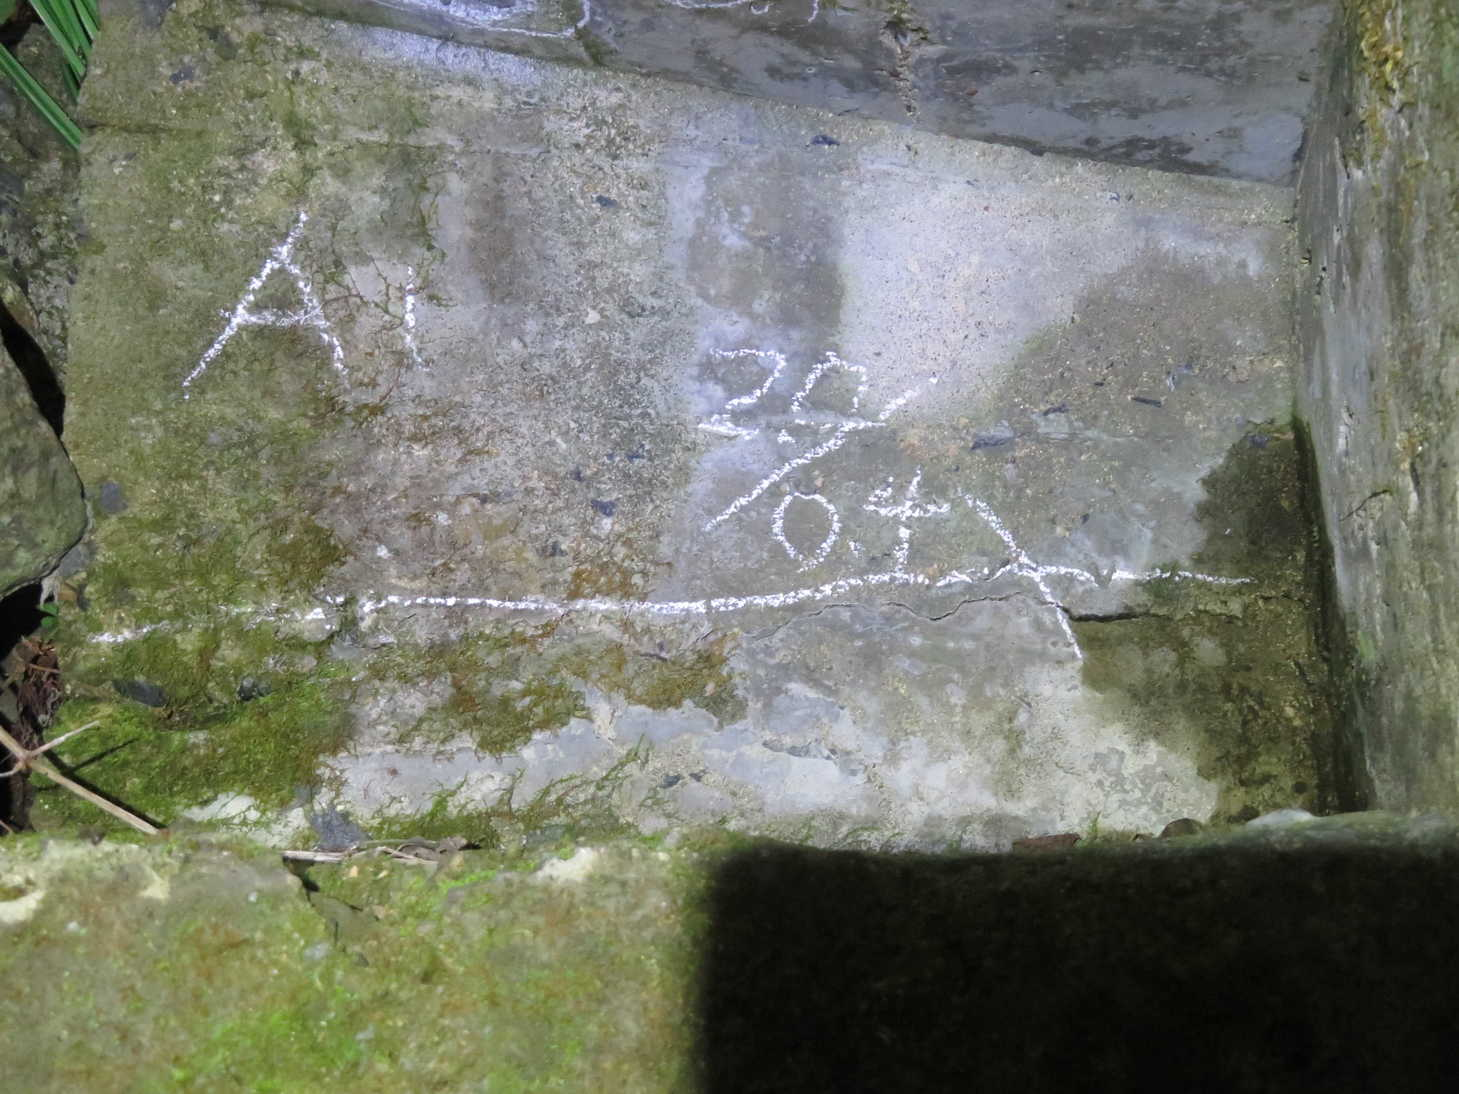
\includegraphics[width=0.75\linewidth]{figures_vlm/s8/s8_10_abutment_cracking.jpg}\par}
    \vspace{2pt}
    {\scriptsize\raggedright
    \textbf{Quality Metrics:}~\textit{Sim(emb):~0.756,\;Sim(tfidf):~0.062}\\[2pt]
    \textbf{GT:} A1abutment cracking(max W=1.2mm); lime efflorescence, P1pier cracking(max W=0.3mm); rust staining lime efflorescence; , A1abutment; P1pier expansion joint \textbf{water leakage} trace observed. cracking rust staining and localized , periodic monitoring;, repair if necessary .\\[2pt]
    \textbf{Pred:} main girder rebar exposure observed. Also, parapet/overhang delamination \textbf{water leakage} is present. parapet delamination , insufficient cover carbonation . localized .
    \par}
  \end{minipage}
  \\[8pt]
  \begin{minipage}[t]{0.46\textwidth}
    {\centering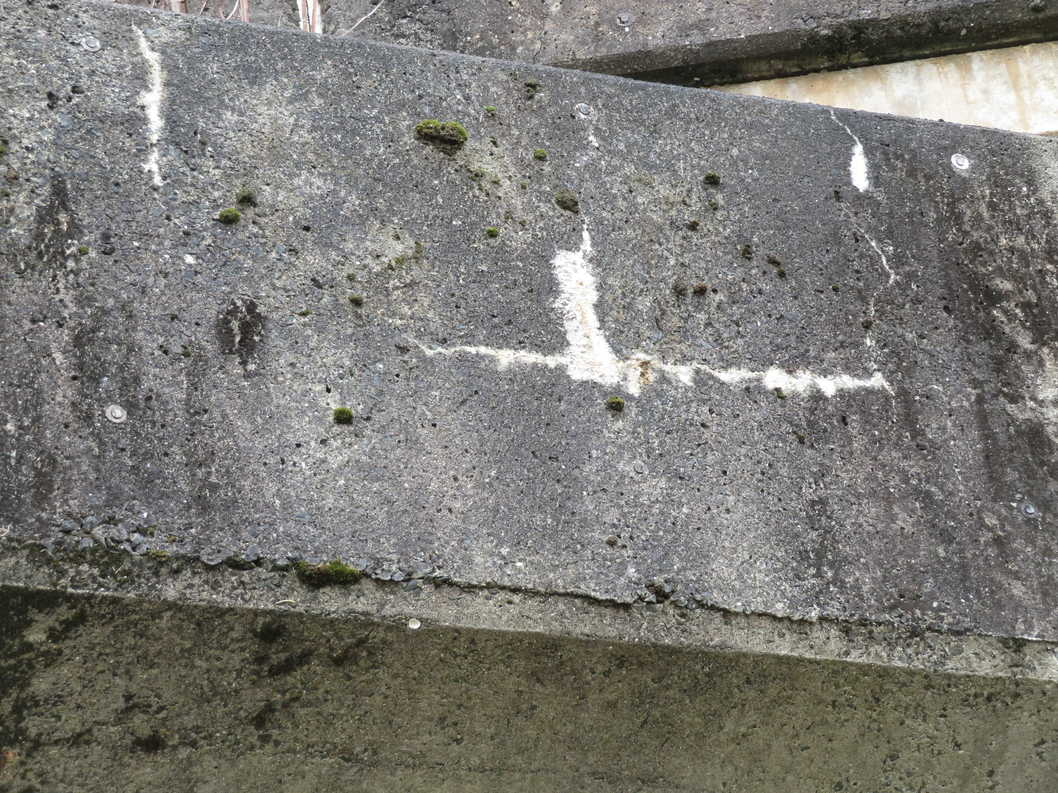
\includegraphics[width=0.75\linewidth]{figures_vlm/s8/s8_11_abutment_rebar_exposure.jpg}\par}
    \vspace{2pt}
    {\scriptsize\raggedright
    \textbf{Quality Metrics:}~\textit{Sim(emb):~0.783,\;Sim(tfidf):~0.178}\\[2pt]
    \textbf{GT:} abutment, pier \textbf{cracking}, \textbf{rebar exposure}, water leakage trace observed. from a durability standpoint,repair is recommended.\\[2pt]
    \textbf{Pred:} main girder \textbf{rebar exposure} observed. Also, generally\textbf{cracking} delamination , expansion joint infiltration water internal rebar expansion .
    \par}
  \end{minipage}
  \hfill
  \begin{minipage}[t]{0.46\textwidth}
    {\centering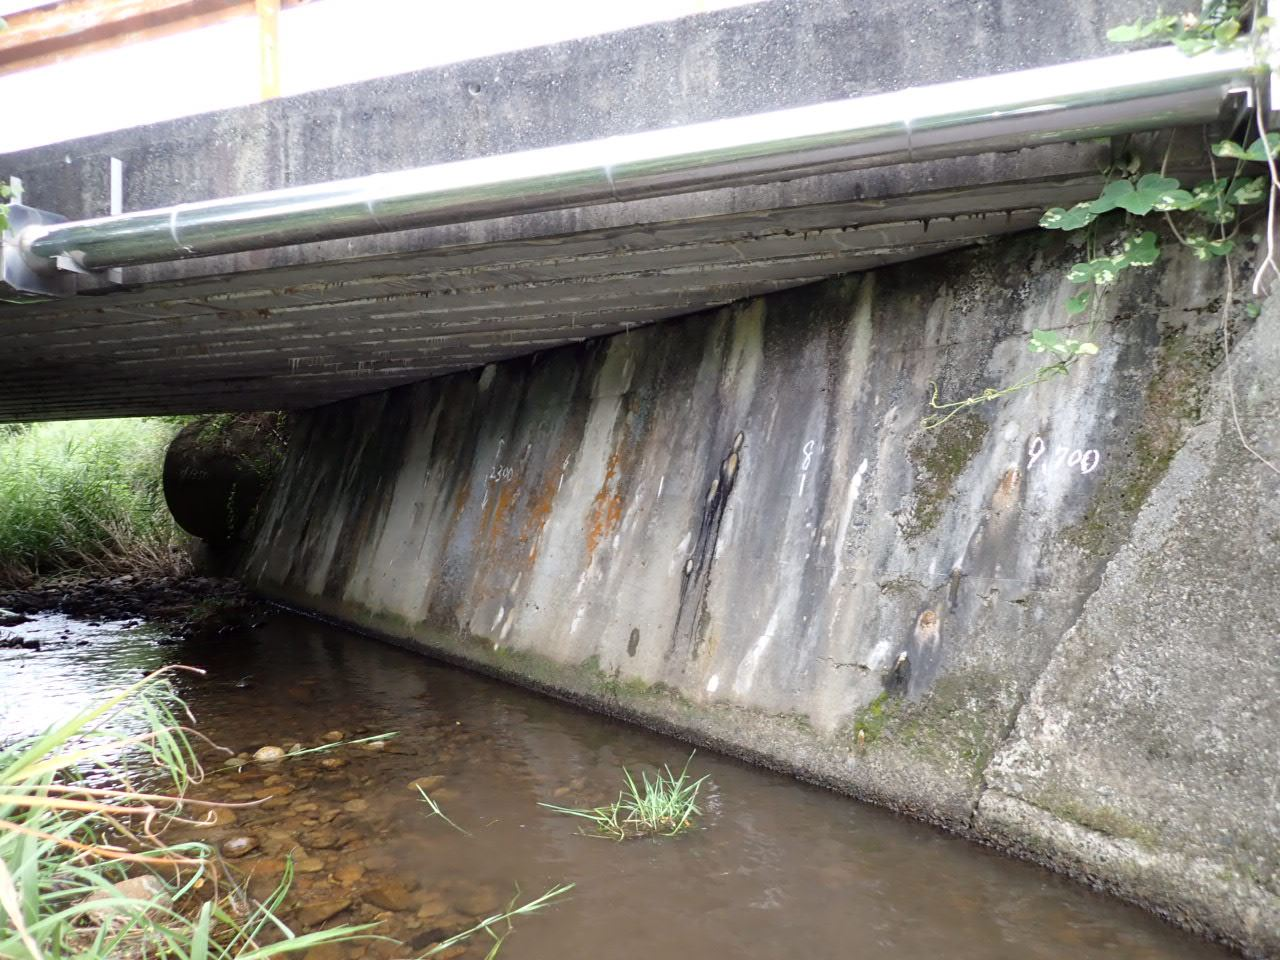
\includegraphics[width=0.75\linewidth]{figures_vlm/s8/s8_12_abutment_spalling.jpg}\par}
    \vspace{2pt}
    {\scriptsize\raggedright
    \textbf{Quality Metrics:}~\textit{Sim(emb):~0.722,\;Sim(tfidf):~0.130}\\[2pt]
    \textbf{GT:} abutment honeycombing spalling is present. \textbf{bearing} soil ejection, lime efflorescence water leakage trace observed. abutment honeycombing , rust staining water leakage trace observed. observed.\\[2pt]
    \textbf{Pred:} main girder rebar exposure, delamination observed. Also, parapet/overhang , expansion joint infiltration water \textbf{bearing} . periodic monitoring;, repair if necessary . , expansion joint infiltration water due to .
    \par}
  \end{minipage}
  \caption{Representative PASS predictions from the v0.7.3 pipeline (3/3). Each panel shows \textbf{GT} (full original inspection record), \textbf{Pred} (full VLM-generated description), and cosine similarities: \textit{Sim(emb)} (sentence-embedding) / \textit{Sim(tfidf)} (TF-IDF). Shared terms are in bold.}
  \label{fig:s8_pass_3}
\end{figure}

\noindent When keywords for structural members and damage types appear in \emph{both} GT and Pred, the Quality Metrics (\textit{Sim(emb)}, \textit{Sim(tfidf)}) are correspondingly high, indicating successful damage recognition. Conversely, when member or damage terms appear only in GT and are absent from Pred, the model has missed key descriptors---representing a recognition gap and an area for future improvement.
